\chapter{Literature Review}

\section{Introduction}
% This introduction is pretty poor, probably best to rewrite once the rest is finished
In this chapter I will give an overview of the existing literature that is appropriate to my project. The chapter is split into two sections. The first section gives a review of Model Driven Engineering and tools that can be used for implementation. The second section investigates software testing methods and ways of assessing the quality of software tests.

\section{Model Driven Engineering}

\subsection{Introduction}
% The Oxford English dictionary defines Model Driven Engineering as... just kidding
Model Driven Engineering is a development methodology that aims to reduce the amount of time spent on code development by building models that can be transformed and used to generate code automatically. This reduces the probability of bugs, as the automatically generated code should contain no bugs (as long as the model is correct). Maintenance time is also reduced, as changes to the system can be implemented by changing a model, and re-generating code \citep{mdseLano}.

In the 1980's there was a software quality crisis that lead to the search for alternative approaches to developing software. Model Driven Engineering is one solution that was of interest at the time as it provided a way to visually represent a system architecture, and from that generate code automatically. However, the return on investment that companies were expecting from model driven engineering was far too high, causing much disappointment and disillusionment, and for a while the concept was sidelined. More recently, the Object Managment Group (OMG) have promoted and developed a Unified Modeling Language (UML), and tools such as Epsilon have further promoted the use of MDE \citep{mdeHistory}.  \citet{brambillaBook} believes that Model Driven Engineering is now past the `trough of disillusionment' and into the `slope of enlightenment' (see figure \ref{mde_pos}) \\

\begin{figure}[p]
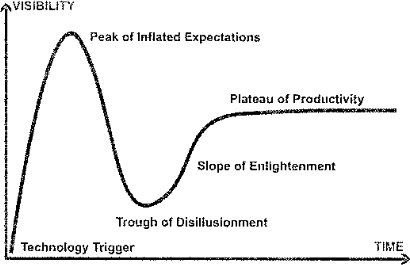
\includegraphics[scale=0.6]{figures/mde_pos.jpg}
\caption{The technology hype cycle according to \citet{brambillaBook}}
\label{mde_pos}
\end{figure}

\subsection{Metamodels}
\subsection{Epsilon}
\subsection{EuGENia}
\subsection{EuGENia Live}

\section{Software Testing}
\subsection{Introduction}
\subsection{Code Coverage}
\subsection{Path Coverage}
\subsection{Test Driven Development}
\subsection{Mutation Testing}

